\section{Postulates and Formalisms}

(\textbf{Notation hint:} For unified symbols, units, and macros, see Appendix~\ref{app:nomenclature}.)

\subsection{P1. Discrete Dynamics and Global Ordering}

The substrate evolves in discrete steps $(T)$. All causality is \textbf{monotonic in $(T)$}.

\subsection{P2. Two Proximities and a Projection}

\begin{itemize}
\item \textbf{$(M)$}: emergent spacetime with metric $(g_{\mu\nu})$, where ordinary matter moves locally and obeys relativity.
\item \textbf{$(S)$: The Pattern Bundle.} We define the total pattern space as a bundle $\tilde{S}$ over the emergent spacetime $M$. For each point $x \in M$, the fiber $S_x$ consists of the equivalence classes of microscopic substrate states supported in a neighborhood of $x$. The total space is $\tilde{S} = \bigsqcup_{x \in M} S_x$.
\item \textbf{$(\pi)$: The Projection.} The map $\pi: \tilde{S} \to M$ is the canonical bundle projection, mapping any pattern $\sigma_x \in S_x$ back to its spacetime location $x$.
\item \textbf{$(d_\sigma)$: Structural Metric.} The distance $d_\sigma$ is defined \textbf{on the fibers}: it measures the algorithmic or structural similarity between two patterns $\sigma \in S_x$ and $\sigma' \in S_{x'}$, independent of their base points $x$ and $x'$.
\end{itemize}

A schematic of the bundle structure is shown in Fig.~\ref{fig:bundle}.

\begin{figure}[t]
\centering
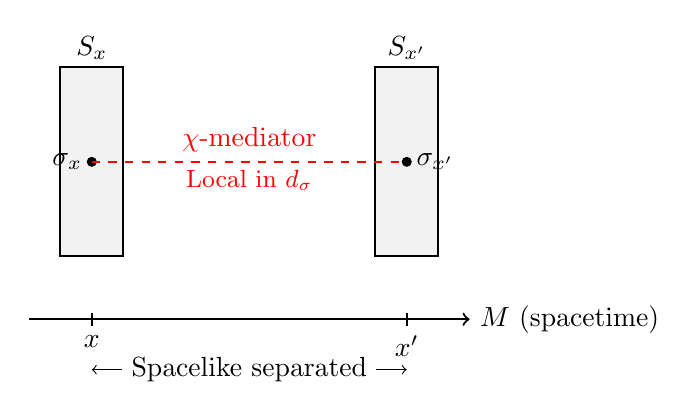
\begin{tikzpicture}[scale=0.8]
  % Base manifold M
  \draw[thick, ->] (-1,0) -- (6,0) node[right] {$M$ (spacetime)};
  \draw[thick] (0,0.1) -- (0,-0.1) node[below] {$x$};
  \draw[thick] (5,0.1) -- (5,-0.1) node[below] {$x'$};
  
  % Fibers S_x
  \draw[thick, fill=gray!10] (-0.5, 1) rectangle (0.5, 4);
  \node at (0, 4.3) {$S_x$};
  \draw[thick, fill=gray!10] (4.5, 1) rectangle (5.5, 4);
  \node at (5, 4.3) {$S_{x'}$};
  
  % Patterns
  \filldraw (0, 2.5) circle (2pt) node[left] {$\sigma_x$};
  \filldraw (5, 2.5) circle (2pt) node[right] {$\sigma_{x'}$};
  
  % Connection in S
  \draw[red, thick, dashed] (0, 2.5) -- (5, 2.5) node[midway, above] {$\chi$-mediator};
  \node[red, font=\small] at (2.5, 2.2) {Local in $d_\sigma$};
  
  % Spacetime separation
  \draw[<->] (0, -0.8) -- (5, -0.8) node[midway, fill=white] {Spacelike separated};
\end{tikzpicture}
\caption{Schematic illustration of the pattern bundle $\tilde S$. Interaction is local in the pattern space fiber (dashed red line) connecting $\sigma_x$ and $\sigma_{x'}$, even though the base points $x, x'$ are spacelike separated in $M$. From the viewpoint of $M$ this appears as superluminal transfer, although every microscopic step is retarded in $\tau$.}
\label{fig:bundle}
\end{figure}

\subsection{P3. Aether Resonance – Substrate-Locality in $(S)$}

There exists a coupling that, within one tick, allows energy or information to move from one region in $M$ to another via a path in $S$ whose cost depends only on $\Dsig(s,s')$, independent of $|\pi(s) - \pi(s')|$ in $(M)$.

\subsection{P4. Conservation Laws in $(M\times S)$}

Total energy/information is conserved over the combined dynamics in $(M\times S)$, even though local budgets in $(M)$ may vary via flows in $(S)$.

\subsection{P5. Substrate classes compatible with our assumptions}
\label{subsec:substrate-classes}

Appendix~\ref{app:assumptions} collects the structural assumptions (A1)--(A9) used in the
derivation of the modified Lieb--Robinson bound, the categorical
causality proof, and the phenomenological estimates.  Here we sketch
what kinds of discrete substrates actually satisfy these assumptions.

\paragraph{Global ordering and strict retardation (A1).}
A1 is satisfied by any discrete--time dynamics in which the microscopic
update rule takes the form
\[
(s,T) \mapsto (s',T+1)
\]
with no backward steps in $T$, and in which the mediator kernel
$G_{\rm ret}$ in $S$ vanishes for $T'<T$.  Concrete examples include
cellular automata on fixed graphs with synchronous updates, and
asynchronous update schemes in which all allowed local moves advance a
global integer ``tick'' $T$ by~1.  In both cases the coarse--grained
substrate time $\tau$ can be taken as a smoothed version of~$T$.
Concrete realizations of such dynamics have been extensively studied in the literature on cellular automata and quantum cellular automata, which provide general frameworks for discrete-time local evolution and for emergent relativistic behaviour~\cite{thooft2016_ca,farrelly2020_qca}. We remain agnostic about the detailed update rule and only assume that it satisfies the structural conditions (A1)–(A9).

\paragraph{Sparsity and weak coupling (A3).}
A3 requires that each node in the substrate pattern graph participates
in at most $g<\infty$ active $S$--edges and that the corresponding
Hamiltonian perturbations $h_e$ obey $\|h_e\|\le\eta$ with
$\mu>\ln g$, where $\mu$ is the decay rate of the kernel in $S$.  This
is naturally satisfied by substrates built from:
\begin{itemize}
  \item locally finite graphs (e.g.\ nearest--neighbour lattices,
        bounded--degree random graphs, sparse small--world networks);
  \item update rules in which only a small fraction of potential edges
        are simultaneously active (e.g.\ stochastic activation with
        fixed mean degree).
\end{itemize}
In such substrates the path sums that enter the function
$\Phi(g,\eta t/\hbar)$ in Eq.~(9.2) converge and the $S$--tail cannot
become distance--independent.

\paragraph{Structure of $O_S$ and degeneracy dilution (A4).}
A4 requires that $O_S$ be constructed from higher--dimension seed
operators with $\Delta>4$, normalized so that $[O_S]=4$, and that
$\langle O_S\rangle$ vanish (or be extremely small) in homogeneous,
periodic, or thermal states because of degeneracy dilution.
Qualitatively, if there are $N\gg 1$ macroscopically equivalent ways to
embed a given mesoscopic pattern into a homogeneous background, then a
generic superposition of those embeddings yields an overlap that
scales as $1/\sqrt{N}$ or smaller.  This drives the effective quality
factor $Q$ to zero in the thermodynamic limit.  Appendix~\ref{app:degeneracy-toy-model} gives an
explicit toy model illustrating this scaling on a finite lattice.

Conversely, in carefully engineered mesoscopic platforms (Sec.~5.3)
the pattern selected by $O_S$ can be realized in only a few locations
with aligned phases, so that $Q$ can approach order unity.  This
difference between ``generic'' and ``engineered'' states is what
suppresses collider and everyday signatures while allowing sharply
tuned experiments to be sensitive.

\paragraph{Kernel structure and minimal Lorentz breaking (A5--A6).}
A5 and A6 are satisfied by substrates in which:
\begin{itemize}
  \item the similarity kernel $K_\sigma(\sigma,\sigma')$ depends only
        on a bona fide metric $d_\sigma(\sigma,\sigma')$ as in
        Eq.~(7.1), with $K_\sigma=\exp[-d_\sigma/\lambda_\sigma]$;
  \item the $u^\mu$ aether/khronon sector lies within the
        Einstein--\ae{}ther / khronometric parameter region where
        $c_T=c$ and preferred--frame effects in gravity obey existing
        bounds [cf.\ Eq.~(3.1C)].
\end{itemize}
In other words, the substrate can carry a preferred frame and an
$S$--metric without spoiling standard tests of GR provided the
aether/khronon sector is chosen conservatively.

\paragraph{Cost monotonicity and pump budget (A2, A8, A9).}
A2, A8, and A9 formalize the idea that resonance steps carry a positive
thermodynamic cost and that the pump budget is finite.  These
assumptions are satisfied whenever:
\begin{itemize}
  \item each microscopic update that changes the $S$--state dissipates
        at least $k_B\Theta\ln 2$ of entropy per bit of information, in the
        spirit of Landauer's principle;
  \item the total pump power $P_{\rm pump}$ is bounded on the relevant
        time scales.
\end{itemize}
Under these conditions we can define a cost functor $\tilde K$ as in
Appendix~D and a pump-rate $\Gamma_{\rm pump}$ as in Sec.~6.2, and the
resource inequality (8.3) follows.

These examples are not meant as a unique substrate proposal; they are
intended to demonstrate that the abstract assumptions (A1)--(A9) are
satisfied by broad classes of discrete systems rather than by a single
fine--tuned construction.

Postulates P1--P4 define the effective framework at the level of spacetime $M$, the substrate time function $\tau$, and the pattern space $S$. For some of our more technical results, in particular the modified Lieb--Robinson bound and the causality statements, we will also use a set of structural assumptions (A1--A9) collected in Appendix~\ref{app:assumptions}. These assumptions constrain the allowed substrates more strongly (for example by requiring sparsity and bounded degree of $S$-links), but they are not needed for the definition of the action or the basic split conservation laws in Sec.~\ref{sec:action}. In later sections we will be explicit about which derivations use only P1--P4 together with (A1)--(A9) and therefore apply to any substrate in this class, and which rely on additional modelling choices introduced below.
